% =====================================================================
%  Tieu su tac gia. Van ban lay tu ban da nop IJNM (paper/paper2/main.tex,
%  cac lenh \authorbio), chi sua duy nhat mot cho: doan cua Quan Tran Anh Vo
%  noi ve "reliability of predictions on rare attacks", ma ban nay da chi ra
%  la khong do duoc -- da doi cho khop voi noi dung that.
%
%  Anh lay tu paper/paper1/authors/ (cung nguoi, cung anh thay dung).
%  Thu tu theo danh sach tac gia tren trang dau.
% =====================================================================

\begin{IEEEbiography}[{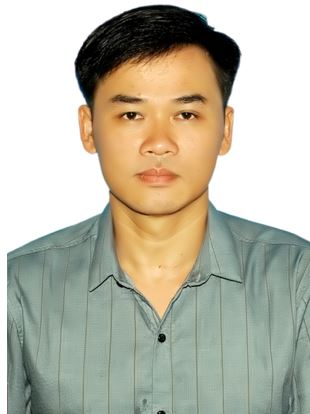
\includegraphics[width=1in,height=1.25in,clip,keepaspectratio]{authors/van.jpg}}]{Nguyen Nang Hung Van}
received the Ph.D. degree in Computer Science from The University of Danang,
Vietnam, in 2021. He is currently a Lecturer with the Faculty of Information
Technology, The University of Danang -- University of Science and
Technology, Danang, Vietnam. His research interests include artificial
intelligence, machine learning, geometric algebra, quantum machine learning,
and computer networking.
\end{IEEEbiography}

\begin{IEEEbiography}[{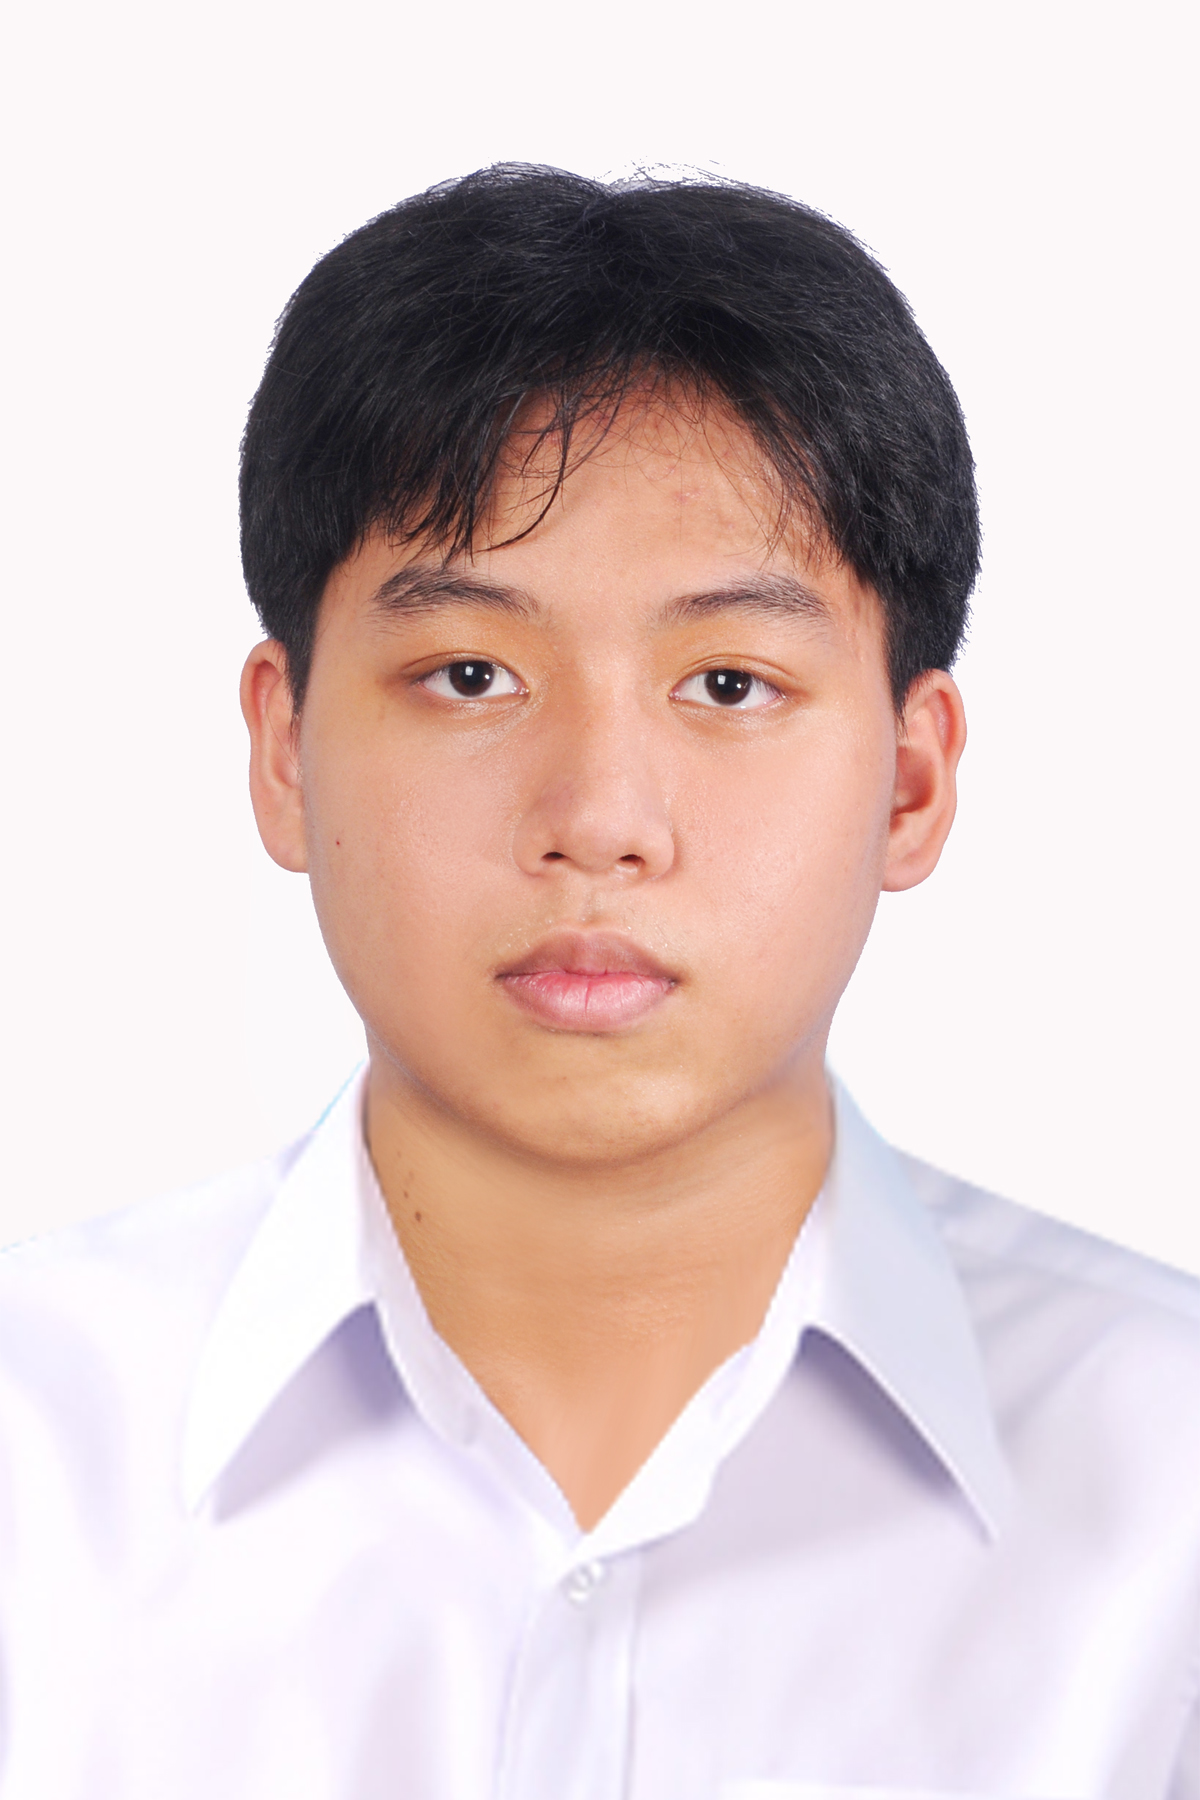
\includegraphics[width=1in,height=1.25in,clip,keepaspectratio]{authors/vo.jpg}}]{Quan Tran Anh Vo}
is currently a third-year undergraduate student pursuing the B.S. degree in
Information Technology, majoring in Data Science and Artificial
Intelligence, with The University of Danang -- University of Science and
Technology, Danang, Vietnam, where he leads this research project. In this
work he established that a binned calibration estimate restricted to a
single attack category is degenerate, designed the measurement protocol
that replaced it, and carried out the cross-dataset and circuit-width
evaluation. His research interests include quantum machine learning and
trustworthy machine learning for network intrusion detection.
\end{IEEEbiography}

\begin{IEEEbiography}[{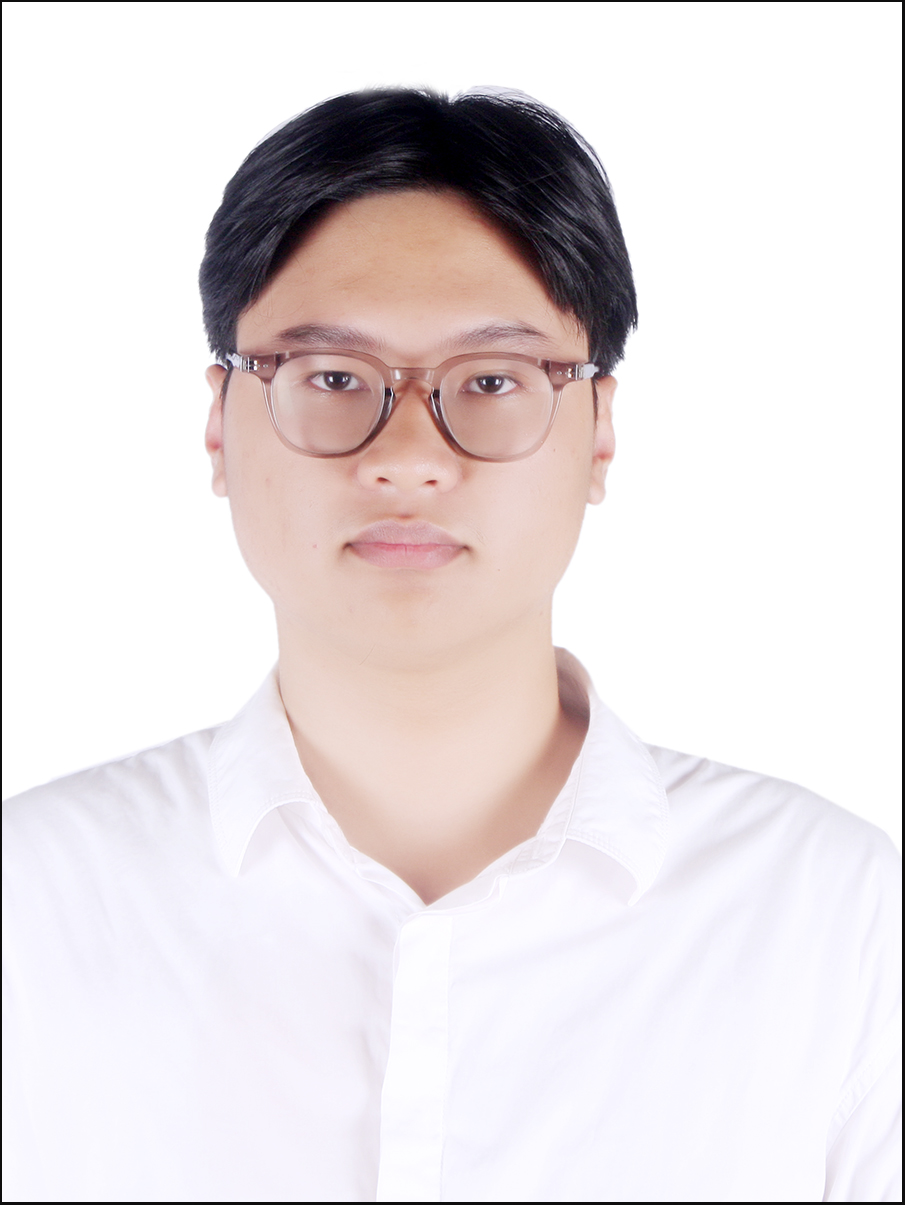
\includegraphics[width=1in,height=1.25in,clip,keepaspectratio]{authors/nguyen.jpg}}]{Nguyen Quang Anh}
is currently a third-year undergraduate student pursuing the B.S. degree in
Information Technology at The University of Danang -- University of Science
and Technology, Danang, Vietnam. He is a member of the research team behind
this study, where he contributed to the experimental evaluation, data
preparation, and analysis of the results. His research interests include
quantum machine learning, machine learning for network security, and network
intrusion detection.
\end{IEEEbiography}

\begin{IEEEbiography}[{
\includegraphics[width=1in,height=1.25in,clip,keepaspectratio]{authors/pham.jpg}}]{Minh Tuan Pham}
received the Ph.D. degree in Computational Science and Engineering from
Nagoya University, Japan, in 2012. He is currently a Lecturer with the
Faculty of Information Technology, The University of Danang -- University of
Science and Technology, Danang, Vietnam. His research interests include
artificial intelligence, soft computing, and geometric algebra, together
with their applications to pattern recognition and data analysis.
\end{IEEEbiography}
